\chapter{Background \& Concepts}
\label{ch:background}

\section{Neural Networks}

\subsection{Fully Connected Neural Networks}

Artificial neural networks are inspired on how neurons behave and interact in the brain. They are computing systems used in field of machine learning to solve problems in multiple fields, one of the biggest ones being computer vision.

Neural networks are composed of artificial neurons which combine their inputs with their internal state, pass that to an activation function, and produce a result. Figure \ref{fig:neuron} shows the definition of a single artificial neuron \cite{nn_def}.

\begin{figure}[thbp]
	\centering
	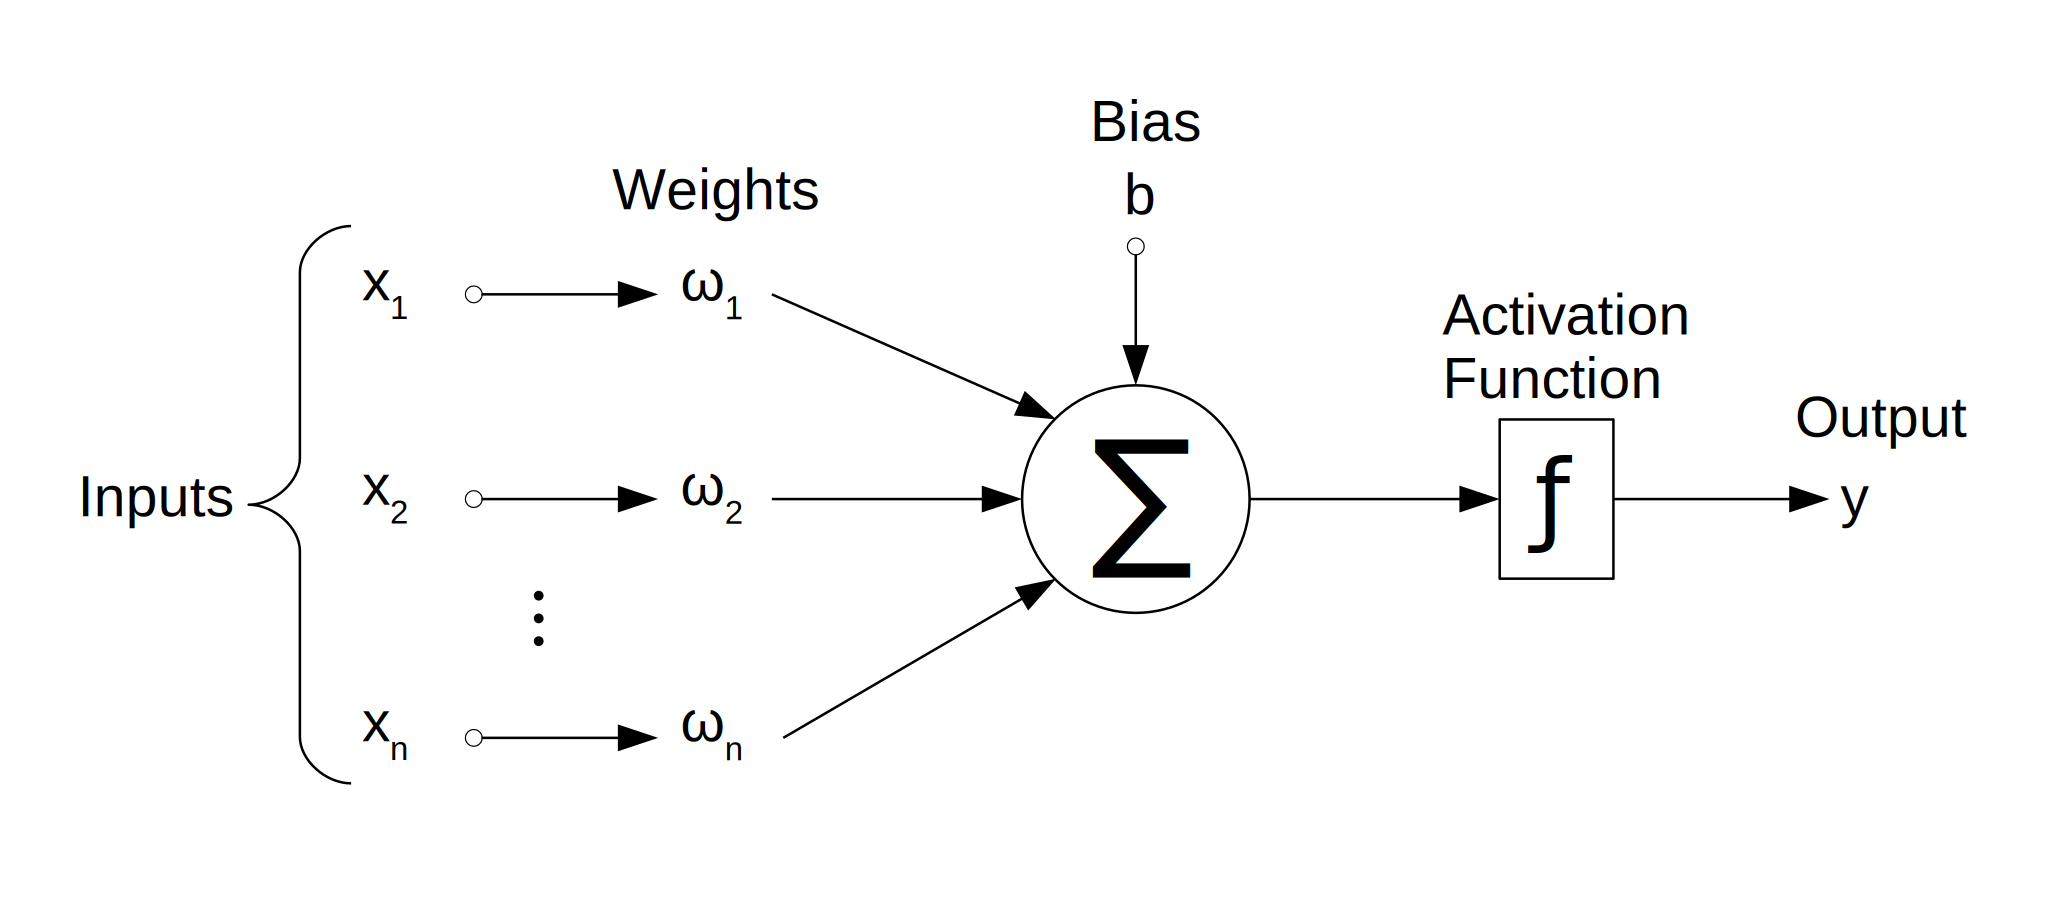
\includegraphics[scale=0.6]{neuron}
	\caption{Artificial neuron definition. Inputs are multiplied by the weights, all that is added together with a bias and passed to an activation function.}
	\label{fig:neuron}
\end{figure}

Multiple neurons stacked define a layer. The outputs from one layer connect to the inputs of another layer to form a neural network. There can be many layers in a single network. The term deep learning comes from the concept of having deep networks, which basically is a network with multiple inner layers. Figure \ref{fig:network} shows a simple network where every output from each layer connects to every input of the next layer. That is called a fully-connected or dense layer \cite{intro_cnn}.

\begin{figure}[thbp]
	\centering
	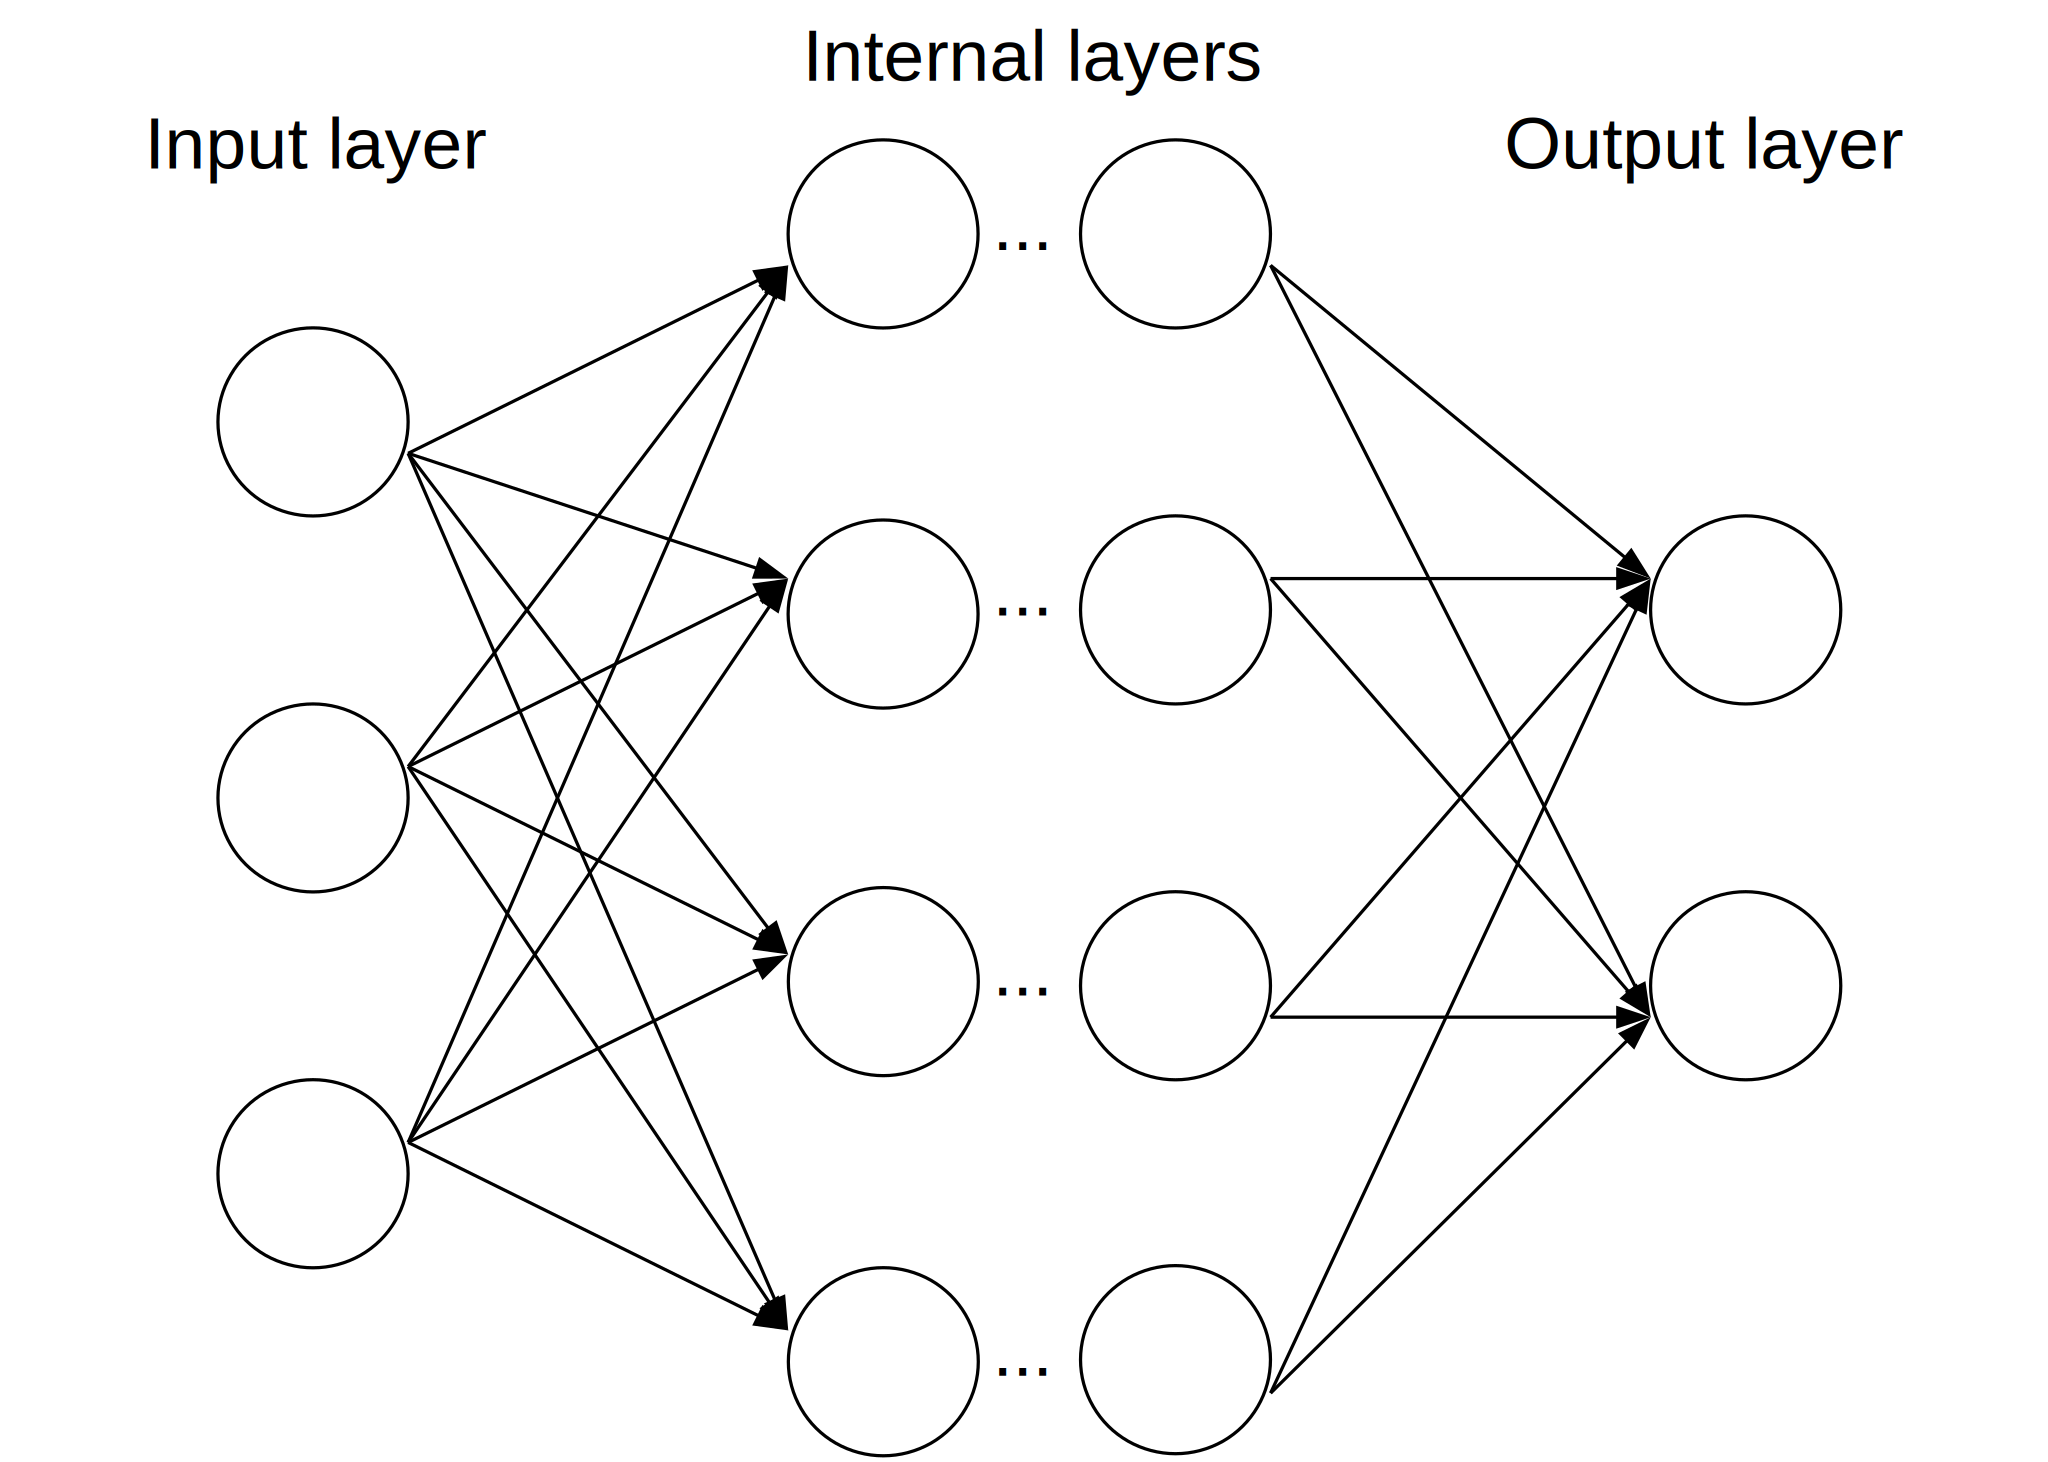
\includegraphics[scale=0.6]{network}
	\caption{Neural network made of fully-connected layers.}
	\label{fig:network}
\end{figure}

To train neural networks the weights and biases of the neurons are tweaked iteratively until the results that the network produces are good enough. On each training iteration the network is given a set of inputs and it will produce a set of outputs. Those outputs are compared against the desired or real values and an error function will produce a numerical value that will tell the network how good or bad was its prediction. That value is then propagated backwards and in each layer the weights and biases of the neurons will be adjusted to minimize the error. This process is called back-propagation.

\subsection{Convolutional Neural Networks}

Convolutional neural networks are a class of deep neural networks that are useful in computer vision fields. They are efficient at analyzing images for applications like image recognition and classification.

CNNs utilize image filters or kernels to do a transformation in a small group of pixels and obtain a result. Kernels are usually a square of a fixed amount of pixels, as typical kernels are 3x3 or 5x5. The kernel is slid through the image and every pixel is multiplied by the kernel weights to produce one pixel for the next layer. Figure \ref{fig:cnn1} shows a visualization of a 3x3 kernel, in this example the pixels in the first layer will be multiplied by the corresponding weights of the kernel and those results will be added together to produce a single value for the next layer \cite{guide_cnn}.

\begin{figure}[thbp]
	\centering
	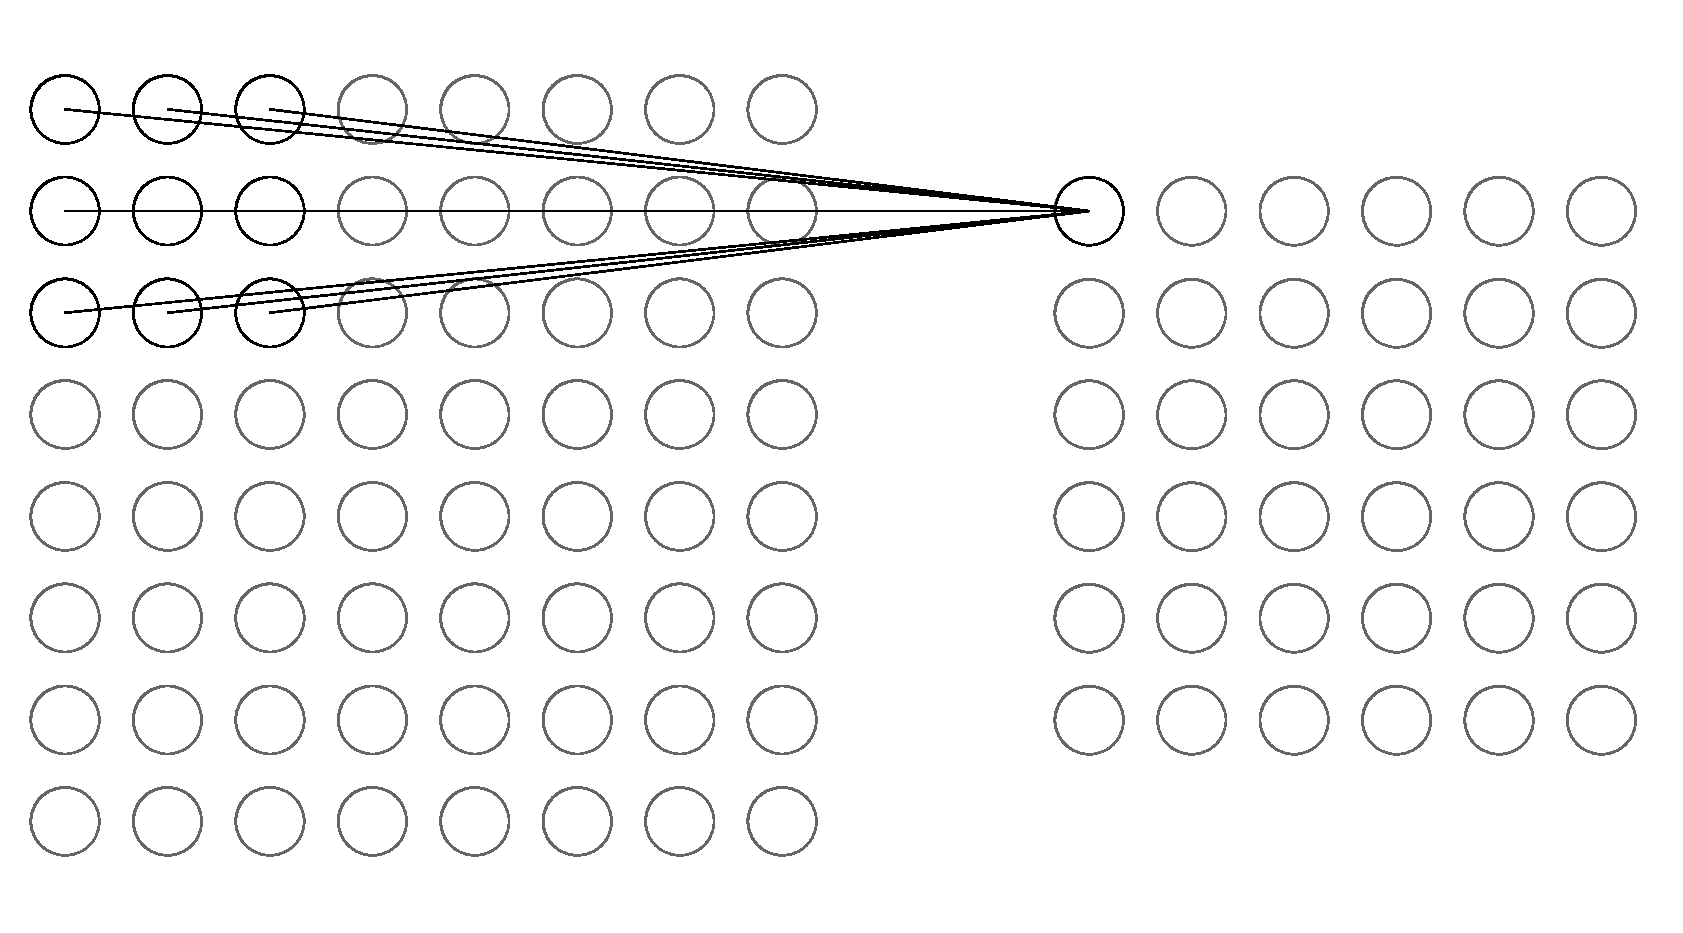
\includegraphics[scale=0.4]{cnn1}
	\caption{Visualization of a 3x3 kernel in a CNN.}
	\label{fig:cnn1}
\end{figure}

CNNs usually utilize multiple kernels at the same time to produce several images in each layer, this gives CNNs depth, which means that CNNs are not actually 2D matrices, but 3D cubes composed of 2D matrices. Usually, each level of depth highlights a special feature of the image, so they are called feature maps but they are also commonly called channels. Figure \ref{fig:cnn2} shows how a convolution layer looks like. In this example, the first layer contains three channels and the next one has five. All the feature maps in the second layer extract information from the first layer \cite{guide_cnn}.

\begin{figure}[thbp]
	\centering
	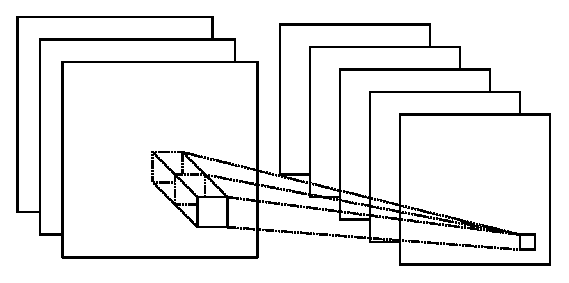
\includegraphics[scale=1.25]{cnn2}
	\caption{Visualization of a convolution layer.}
	\label{fig:cnn2}
\end{figure}

Due to of how CNNs work, the trivial example of having a 1x1xC1 (height=1, width=1, channels=C1) layer followed by a 1x1xC2 layer and using a 1x1 kernel is the same as having a simple layer of \textit{C1} number of inputs followed by a fully-connected layer of \textit{C2} number of neurons. If the 1x1 kernel is kept but the layer dimensions are changed to an arbitrary height (H) and width (W) it would be the same as having HxW individual fully-connected layers. This can be exploited to run several full-connected neural networks in parallel in neural accelerators that are optimized for CNNs.

\subsection{Software-Level Optimizations and Approximations for Neural Networks}

\subsubsection{Pruning}

Pruning is the process of taking a neural network and removing some amount of neurons and/or connections (synapses). Usually this process is done intelligently by analyzing which neurons have weights close to zero and which connections affect the least the accuracy of the network. Once these neurons are identified the weights and biases are set to zero or removed completely from the network. Pruning can be done as a post-training optimization or it can be done during training \cite{prune1}.

Figure \ref{fig:prune} shows an example of how a neural network might look like before and after it is pruned. Pruning a neural network can have several positive effects. The network itself can be compressed and the file size is reduced. If the connections and neurons are removed completely the network itself is reduced in size and less operations need to be calculated when running the network. If the neurons are not removed and just zeroed the network might still run the operations, but if the hardware and/or software environment supports it, these zero weights can be identified and the operations can be skipped.

\begin{figure}[thbp]
	\centering
	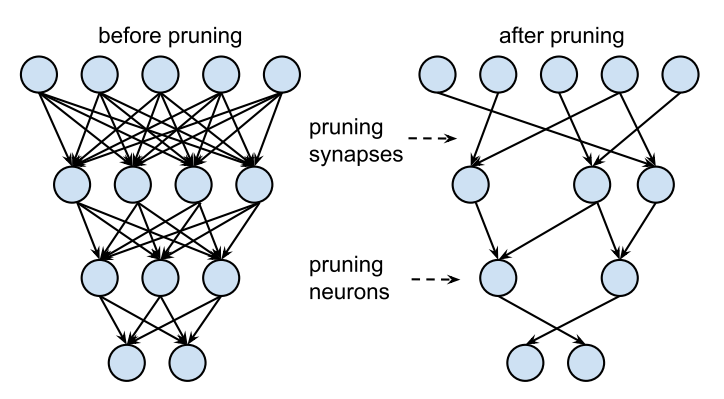
\includegraphics[scale=0.5]{prune}
	\caption[Example of neural network before and after pruning.]{Example of neural network before and after pruning \cite{Han2015}.}
	\label{fig:prune}
\end{figure}

\subsubsection{Separable Convolution}

Sliding a kernel through a CNN requires many operations, and it increases dramatically when the depth of the CNN is large. Let's take the example of a CNN where the input image is 12 by 12 pixels, the kernel is 5 by 5, it has three channels, a stride is one and there is no padding (this sets the next layer size to 8 by 8 pixels). Let's also assume that the next convolutional layer has a depth of 256. If a normal convolutional layer is used, this means that a 5x5x3 kernel is slid through the image 256 times, which means that a total of 5x5x3x8x8x256=1,228,800 operations need to be done, see Figure \ref{fig:normal_conv}.

\begin{figure}[thbp]
	\centering
	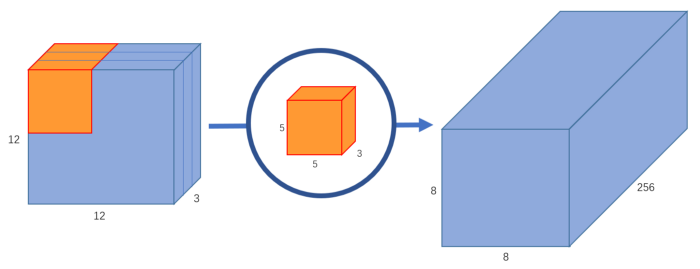
\includegraphics[scale=0.5]{normal_conv}
	\caption[Normal convolution example.]{Normal convolution example \cite{sep_conv}.}
	\label{fig:normal_conv}
\end{figure}

A normal convolution can be separated in two stages: a depthwise convolution and a pointwise convolution. Following the previous example, the depthwise convolution would have three kernels of shape 5x5x1 slid through the input image to create a 8x8x3 image, see Figure \ref{fig:depth_conv}. The output that we are seeking is 8x8x256, so now a pointwise convolution will be applied to make that shape. This means that 256 1x1x3 kernels will be applied to the 8x8x3 image created by the depthwise convolution and the result will be the desired 8x8x256 image, see Figure \ref{fig:point_conv}. The depthwise convolution needs 5x5x3x8x8=4,800 operations to be calculated and the pointwise convolution needs 1x1x3x8x8x256=49,152 operations. In total the separable convolution needs 53,952 operations, a much lower number than the normal convolution.

\begin{figure}[thbp]
	\centering
	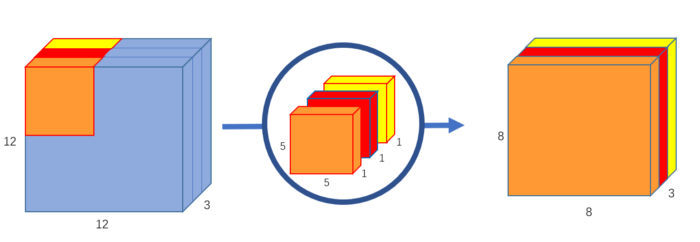
\includegraphics[scale=0.5]{depth_conv}
	\caption[Depthwise convolution example.]{Depthwise convolution example \cite{sep_conv}.}
	\label{fig:depth_conv}
\end{figure}

\begin{figure}[thbp]
	\centering
	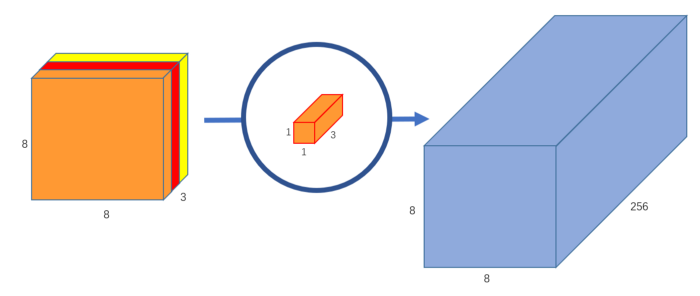
\includegraphics[scale=0.5]{point_conv}
	\caption[Pointwise convolution example.]{Pointwise convolution example \cite{sep_conv}.}
	\label{fig:point_conv}
\end{figure}

Conceptually, in a normal convolution the image is transformed 256 times, each time this is done 4,800 multiplications are needed. In the case of the separable convolution the transformation is done only once, during the depthwise convolution, so basically the transformed image is taken and it's just elongated to a depth of 256. This saves computational power since the image doesn't need to be transformed multiple times \cite{sep_conv}.

\subsubsection{Quantization}

In neural networks quantization is the concept of converting the weights in the neurons from a type with more precision to another type with less precision. Depending on the hardware, floating point operations can be slower and more power hungry than integer operation, so usually the process involves the conversion from floating point to integer. The quantization process is done to optimize the networks to run in hardware where integer operations can be executed faster and with less energy. Quantization doesn't only involve converting from floating point to integer, another optimization is to reduce the amount of bits for each weight, this can significantly accelerate the performance and energy efficiency of the network, specially if the hardware supports executing vector operations where several integer operations can be execute in parallel. The downside of quantization is that integer types can represent a lower range of numbers which means that when doing the computations precision is lost. If not done carefully quantizing a neural network can result in a significant loss of accuracy \cite{quant1}.

\section{Accuracy Estimation}

There are several methodologies on how to measure the error of results. In this section three different methods will be defined. These methods will be used in other chapters to measure the accuracy of the results obtained.

\subsection{Mean Absolute Percentager Error (MAPE)}

The first step to calculate this type of error consists in taking the absolute error for each measurement and dividing it by the corresponding expected (actual) value, this generates the relative error for each individual measurement. Then the sum of all the relative errors is taken and divided by the total number of measurements, generating the mean of all the relative errors \cite{DeMyttenaere2016}.

The formula that defines this error is the following:

\begin{equation}\label{eq:mape}
MAPE=\frac{1}{n}\sum_{t=1}^{n}\left| \frac{A_{t}-F_{t}}{A_{t}} \right|
\end{equation}

Where $A_t$ is the actual (real/expected) value and $F_t$ is the forecast (measured) value.

Although very popular and simple, this way of measuring error has some issues. Problems with this calculation start to be evident when the denominators are relatively small or zero. Checks need to be added when doing the calculations in order to avoid dividing by zero, in which case the error is set to 1 (100\%). Also, when the forecast values are too low, the percentage error can't exceed 100\%, but when they are too high there is no upper limit.

\subsection{Weighted Mean Absolute Percentage Error (WMAPE)}

This is an alternative to MAPE that alleviates the issue of small or zero denominators. It does it by separating the sums and calculating the absolute error of all the measurements first and then dividing by the sum of all the actual values. Another way of viewing this is substituting the $A_t$ denominator in formula \ref{eq:mape} with the average of all the actual values in the series \cite{wmape}.

\begin{equation}\label{eq:wmape}
WMAPE=\frac{1}{n}\frac{\sum_{t=1}^{n}\left| A_{t}-F_{t} \right|}{\sum_{t=1}^{n}A_{t}}=\frac{1}{n}\sum_{t=1}^{n}\left| \frac{A_{t}-F_{t}}{\bar{A}_{t}} \right|
\end{equation}

Were

\begin{equation}\label{eq:actual_vals_average}
\bar{A}_{t}=\frac{1}{n}\sum_{t=1}^{n}A_{t}
\end{equation}

The only disadvantage of this error measurement is that it can potentially hide or smooth out a small amount of big errors due to the averaging of the denominators.

\subsection{Mean Squared Error (MSE)}

This error calculates the mean of the squares of the absolute errors. It follows the following formula \cite{mse}:

\begin{equation}\label{eq:mse}
MSE=\frac{1}{n}\sum_{t=1}^{n}\left( A_{t}-F_{t} \right)^{2}
\end{equation}

This error measurement is good at showing big errors and at the same time hiding small errors, all this due to the squaring. The disadvantage is that the final measurement is absolute, not relative. This means that it is not suitable for comparing against other applications where the data range could be different.

\section{The OpenVINO Toolkit}

OpenVINO is a toolkit that facilitates programmers to utilize Intel hardware to do inference of neural network models. There are two main components to the toolkit: the Model Optimizer and the Inference Engine.

The Model Optimizer is a tool that facilitates the transition between the training and deployment environment. It performs model analysis and transforms the models for optimal execution in Intel hardware. It is composed of a series of scripts that take as input a saved model in one of the supported formats. The Model Optimizer can transform models from the following frameworks: Caffe, Tensorflow, MXNet, Kaldi and ONNX. The output of the Model Optimizer is called the Intermediate Representation (IR) of the network. The IR is composed of a pair of files that describe the mode: an XML file that describes the topology of the network and a binary file that contains the weights and biases of the neurons. Once the IR file is generated, it can be loaded onto a piece of hardware using the Inference Engine \cite{openvino_toolkit}.

\begin{figure}[thbp]
	\centering
	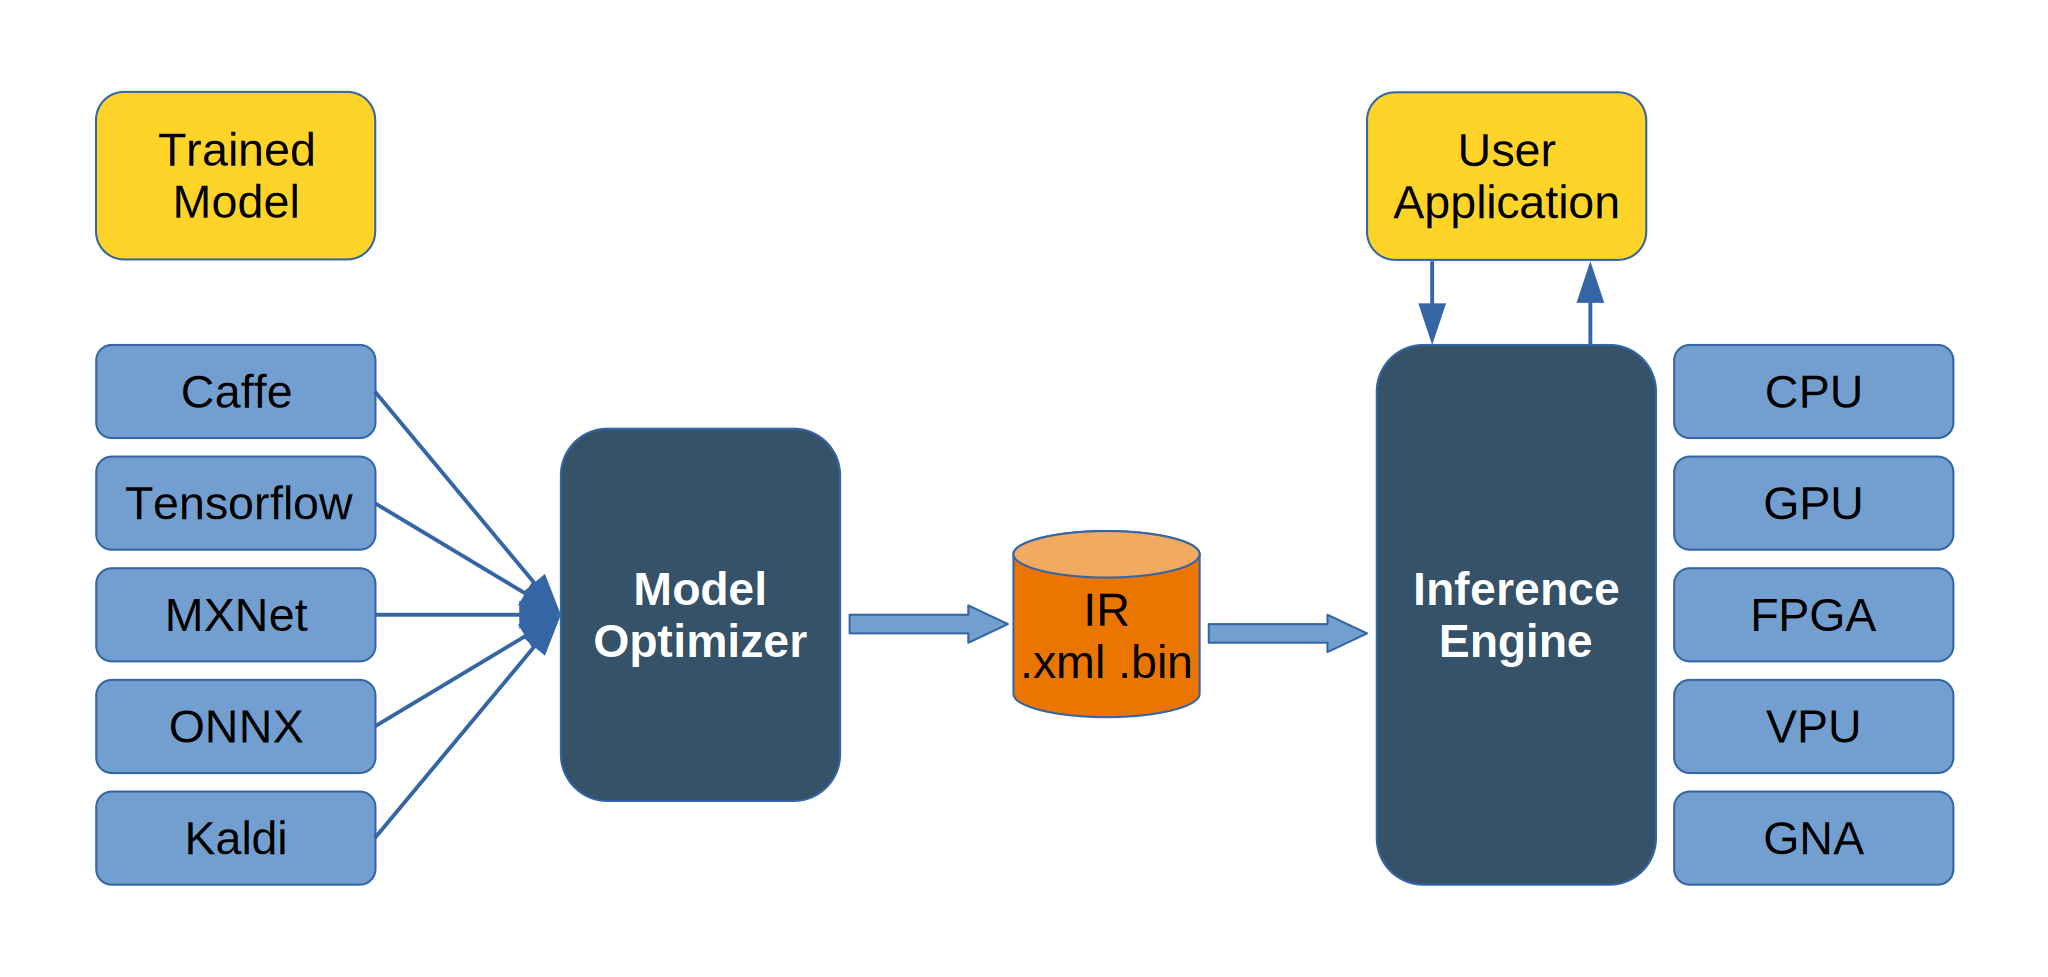
\includegraphics[scale=0.55]{openvino}
	\caption[OpenVINO workflow.]{OpenVINO workflow \cite{openvino_toolkit}.}
	\label{fig:openvino}
\end{figure}

Summary of the common workflow for using the Inference Engine API:

\begin{enumerate}
    \itemsep0em
	\item Create Inference Engine Core object
	\item Read the Intermediate Representation 
	\item Prepare inputs and outputs format
	\item Compile and Load Network to device
	\item Set input data
	\item Execute
	\item Get the output
\end{enumerate}
\item

The Inference Engine is a set of C++ libraries that provide an API to do inference on the different supported platforms (CPU, GPU, VPU, FPGA or GNA), it even supports heterogeneous inferencing using different pieces of hardware at the same time. The process of using the libraries to do inferencing requires the following steps. First, the user needs to create a \textit{core} object and load the IR files of the model. Then the network needs to be compiled and loaded into the target device. After that an \textit{infer request} object needs to be created, this will have a method called \textit{Infer} that will tell the hardware to act on the input data. Finally, the inputs and outputs need to be defined, an input and an output buffer are created. For each inference the input buffer needs to be filled with the input data and once the inference is done, the results can be accessed through the output buffer and the output data can be copied somewhere else for future use or can be analyzed in place and discarded \cite{openvino_toolkit}.
